In cele ce urmeaza voi prezenta solutia software propusa pentru managementul bazelor de date in maniera descrisa anterior. Voi trece in revista arhitectura software, urmand apoi sa explic fiecare din componentele aplicatiei, precum si modul de interactionare a acestora.
\\

\section{Arhitectura Sistemului Software}
Sistemul este impartit in 3 componente importante:
\begin{itemize}
\item Scripturi UNIX ce interactioneaza cu instantele de baze de date;
\item RESTful API folosit pentru a expune functionalitatea oferita de scripturi prin intermediul protocolului HTTP;
\item Aplicatie Web ce comunica prin intermediul protocolului HTTP cu API-ul RESTful expus.
\end{itemize}
In \textit{Figura 2} este prezentata diagrama arhitecturii software.
\begin{figure}[h]
	\centering
	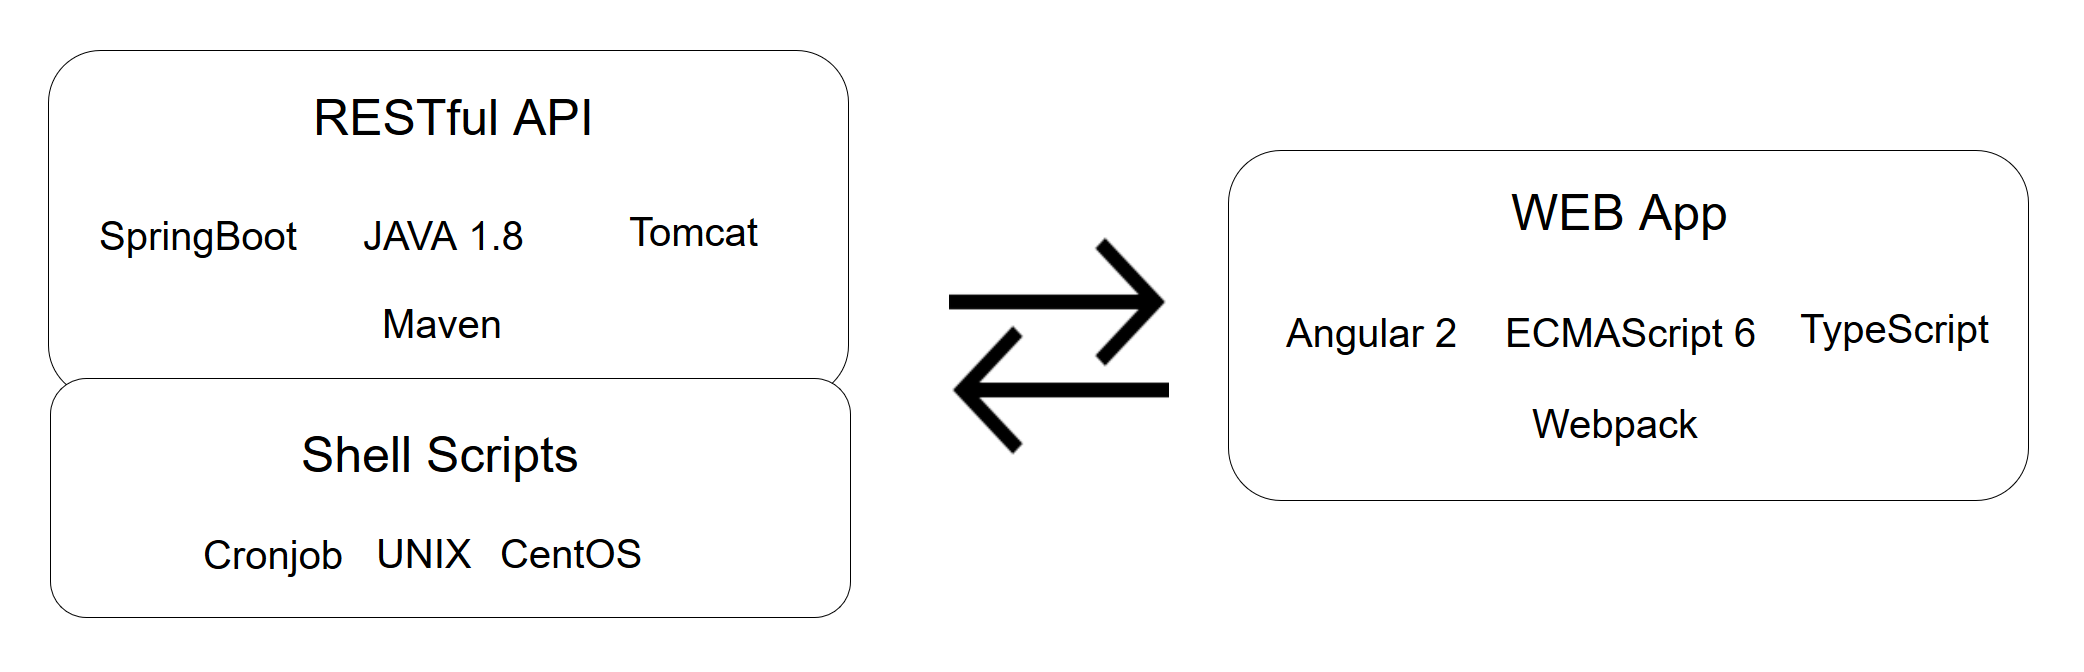
\includegraphics[scale=0.30]{LayeredArchLandscape}
    \caption{Diagrama arhitecturii software}
    \label{fig:LayeredArchPortrait}
\end{figure}
\newpage
\section{Scripturile UNIX}
Functionalitatea de baza a aplicatiei consta in interactionarea cu instantele de baze de date. Pentru asta am facut 3 scripturi ce au urmatoarele responsabilitati:
\begin{enumerate}
\item \textbf{pg-script.sh} pentru interactionarea cu instantele (pornire, oprire, interogare status);
\\
\begin{listing}[ht]
\inputminted[
frame=lines,
framesep=2mm,
baselinestretch=0.9,
fontsize=\footnotesize,
fontfamily=courier,
linenos
]{bash}{sourceCode/pg-script.sh}
\caption{\texttt{pg-script.sh}}
\label{cod:pgScript} 
\end{listing}
\item \textbf{basebackup.sh} pentru crearea de basebackup a unei instante (checkpoint de la care sa se poate incepe procesul de restaurare);
\\
\begin{listing}[ht]
\inputminted[
frame=lines,
framesep=2mm,
baselinestretch=0.9,
fontsize=\footnotesize,
fontfamily=courier,
linenos
]{bash}{sourceCode/basebackup.sh}
\caption{\texttt{basebackup.sh}}
\label{cod:basebackup} 
\end{listing}
\item \textbf{recovery.sh} pentru initierea procesului de restaurare a bazei de date
\\
\begin{listing}[ht]
\inputminted[
frame=lines,
framesep=2mm,
baselinestretch=0.9,
fontsize=\footnotesize,
fontfamily=courier,
linenos
]{bash}{sourceCode/recovery.sh}
\caption{\texttt{recovery.sh}}
\label{cod:recovery} 
\end{listing}
\end{enumerate}\
\par
Toate cele trei scripturi au fost gandite cu scopul de a se crea symbolic links (scurtaturi) catre ele. Acestea vor avea numele instantei bazei de date, iar scriptul principal foloseste numele fisierului scurtatura pentru a accesa datele instantei respective. Scopul este acela de a crea un singur set de scripturi, iar daca avem n instante de baza de date doar creem symbolic links catre scripturi, fiecare cu numele instante de baza de date respective.
\newpage
\section{Server-ul: RESTful API}
Pentru partea de server (backend) a fost aleasa solutia crearii unui RESTful API cu scopul de a se expune functionalitatea oferita de catre scripturile bash prezentate anterior. Am utilizat Java Enterprise Edition, framework-ul Spring, ce facilteaza crearea unui API prin intermediul librariilor SpringWeb.
\par
Un alt motiv pentru care am ales Spring a fost suportul oferit pentru a injecta dependinte urmand sablonul de proiectare Dependency Injection. Astfel, am decuplat controller-ul REST ce primeste cererea web de catre serviciul care o executa. Se poate injecta orice implementare de serviciu in controller, iar codul acestuia nu trebuie schimbat. Versiunea de Java utilizata este 1.8.
\begin{listing}[ht]
\inputminted[
frame=lines,
framesep=2mm,
baselinestretch=0.9,
fontsize=\footnotesize,
fontfamily=courier,
linenos
]{java}{sourceCode/DatabaseManagementAPI.java}
\caption{\texttt{DatabaseManagementAPI.java}}
\label{cod:DatabaseManagementAPI} 
\end{listing}
\newpage
Pentru managementul dependintelor si crearea artefactului s-a folosit Maven. Se ofera ca si exemplu fisierul \textbf{pom.xml}:
\begin{listing}[ht]
\inputminted[
frame=lines,
framesep=2mm,
baselinestretch=0.9,
fontsize=\footnotesize,
fontfamily=courier,
linenos
]{xml}{sourceCode/pom.xml}
\caption{\texttt{pom.xml}}
\label{cod:pom} 
\end{listing}

\newpage
\section{Interfata grafica cu utilizatorul}
Scopul proiectului este crearea unei aplicatii care sa faciliteze manipularea serverelor de baze de date PostgreSQL de catre dezvoltatori care nu trebuie sa aiba acces la masinile pe care se afla bazele de date/ cunostinte de UNIX. In acest sens, avand deja server-ul de Java care expune prin servicii Web functionalitatile respective, trebuie apelate si oferite intr-o maniera cat mai intuitiva. 
\par
Ca si framework am folosit Angular 2, limbajul de programare fiind Javascript, standardul ECMAScript6, impreuna cu TypeScript. Angular 2 are urmatoarele avantaje:
\begin{itemize}
\item este un framework open-source JavaScript construit și întreținut de Google, ceea ce usurează dezvoltarea aplicațiilor web.
\item standardizează aplicațiile la nivel de client (browser), oferind o structură robustă și ușor de implementat în dezvoltarea site-urilor.
\item este alegerea potrivită pentru orice aplicație web, în special dacă se preferă efectele vizuale spectaculoase. Rezultatul este un site fluid și rapid. Acesta este motivul pentru care se pretează SPA-urilor (Single Page Application) și aplicațiilor web destinate dispozitivelor mobile.
\item se integrează ușor cu Bootstrap, permite crearea de aplicații responsive care pot fi accesate atât din browserul calculatorului cât și de pe dispozitivele mobile. Astfel, este ușor să creezi o singură aplicație web care să se vadă perfect pe orice dispozitiv de pe care este accesată – PC, tabletă, telefon, plasmă.
\end{itemize}
\par Ca si manager de pachete am utilizat \textbf{npm} de la NodeJS.
\newpage
\section{Setarea aplicatiei in Amazon Web Services}
Avand ca si obiectiv crearea unui mediu cat mai apropiat de cel aflat pe masinile din productie, am inchiriat un server EC2 de la Amazon.
\par
Sistemul de fisiere a fost stabilit conform descrierii din Capitolul 2. Am inchiriat 3 discuri EBS(Elastic Block Storage) pe care le-am configurat precum a fost prezentat, pentru a seta 3 instante de baza de date.
\par 
Odata ce sistemul de fisiere a fost configurat, am creat scripturile ce vor interactiona cu bazele de date. Urmatorul pas a fost pornirea celor doua servere (backend si frontend). In timpul acestui proces a fost necesara configurarea unui rol de securitate oferit masinii de calcul EC2, pentru a permite traficul pe portul 3001 utilizat de aplicatia frontend.